% vim:ft=tex

\section{Data Prediction with MLPRegressor}\label{sec:mlp}
Since we wanted to implement the prediction algorithm in Python we used the library \emph{Scikit Learn} which provides a class \emph{\acf{mlp}} with according functions.
As we wanted to train a non-linear model we decided to use a Multi-layer Perceptron since it can learn a non-linear function approximator for either classification or regression. However  a \acs{mlp} uses backpropagation which is the most widely used algorithm for supervised learning with multi-layered feed-forward networks \cite{riedmiller1993direct} this algorithm was implemented to train a prediction model for the rental bike usage on a daily base.\\\\
The outcome of of the Data Profiling Part 2, as described in chapter \ref{sec:mlp} served as a basis for the prediction.
As a first implementation we used the following data as an input for the feature matrix: \emph{Month, Weekday, Day, Season, Daily Weather, Daily Weather Past, Humidity, Humidity Past, Windspeed, Windspeed Past, Apparent Temperature (Avg), Apparent Temperature (Avg) Past, Reted Bikes}. Since we assume that weather conditions play an important role in bike usage we decided to add weather data. Another assumption was that on weekdays the frequency will rise, because a lot of people use rented bikes to travel to work. Furthermore we added the number of rentals of today in order to predict the ones of tomorrow. Therefore \emph{Rented Bikes Future} serves as our target variable which is to predicted.\\
Since the \acs{mlp} works with works with data represented as dense and sparse numpy arrays of floating point values, data has to be encoded accordingly. Therefore we mapped all of the ordinal scaled data like \emph{Month, Weekday, Season, Daily Weather} to numerical data, by implementing a dictionary which assigns numerical values to ordinal data. For the weekdays for example we used the following dictionary:
\begin{lstlisting}[language=bash,breaklines=true]
"Weekday": {"Monday": 1, "Tuesday": 2, "Wednesday": 3, "Thursday": 4,"Friday": 5, "Saturday": 6, "Sunday":7 }
\end{lstlisting}
After the encoding we split the data into 80 \% training data and 20\% test data.
Since the \acs{mlp} is sensitive to feature scaling we normalized the data accordingly to the activation function. Since we used the \emph{logistic} activation function which expects vaues bettween [0,1] we normalized the feature matrix as well as the target variable beforehand. Scikit Learn provides several scaling mechanism to rescale the data. 
After data was scaled we applied the \acs{mlp} with \emph{logistic} as an activation function and ten hidden layers with 5 neurons. After the predicton we denormalized the data back to its originally state. In order  the rate the accuracy of the prediction we computed the \acf{rmse} which measures the difference between actual and predicted values by a model, the less the difference respectively the value, the better is the model.
To get a better impression of how the prediction worked, the results were plotted as time series.
The time seres was plotted of for years this causes that the plot was very large. In order to make it more user friendly, we imlemented an interactive plot which gives the user the oportunity the zoom into specific parts or cut out some parts to look at them more closely.\\
In the first attempt we used the \emph{MinMaxScaler} which rescales the data such that all vales are in the range of [0,1].
This gave as an \acs{rmse} of 122.347. To get a better impression of what that means we plotted this result which can be sen in figure \ref{fig:mlpquantile}.
\begin{figure}[H]
\hspace{-2.8cm}
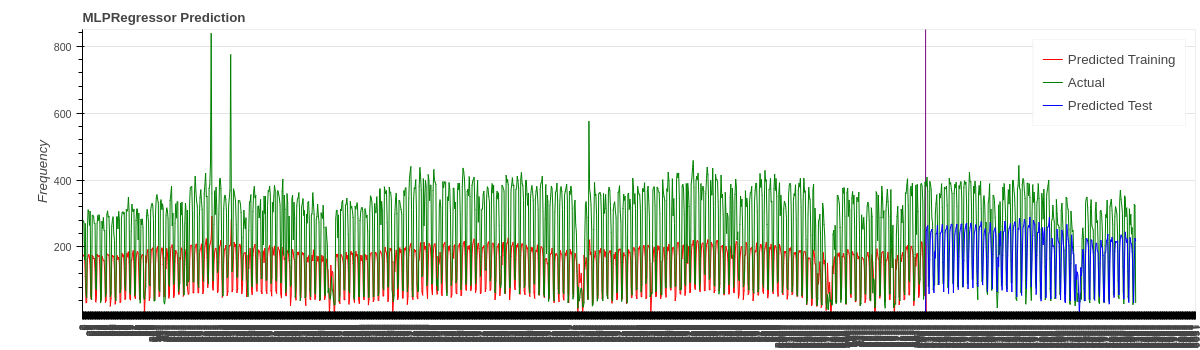
\includegraphics[width=1.4\textwidth]{img/mlpminmax}\label{fig:mlpminmax}
\captionof{figure}{Result of \acs{mlp} with MinMaxScaler}\label{fig:mlpminmax}
\end{figure}
This result shows that the prediction lack accuracy. As we found out this was caused by the MinMaxScaler since this scaler is very sensitive to the presence of outliers. Therefore we chose another scaler for normalization which is more prone to outliers like the \emph{QuantileTransformer} or \emph{MaxAbsScaler}. Experiments were made with all available scalers of Scikit Learn which met the requirements for the output of the scaling. The best result was achieved by the QuantileTransformer with an \acs{rmse} of 57.837, therefore we stuck with this normalization method.\\
Further experiments were carried out in order to evaluate the features. As mentioned earlier the previous predictions were made with a feature matrix of thirteen features. To evaluate which features improve the prediction and which are useless 18 test cases were carried out. Each test case consisted of different constellations of features. In the ed the different \acs{rmse} values were compared, which can be seen in figure \ref{fig:evalmlp}.
\begin{figure}[H]
\hspace{-1.5cm}
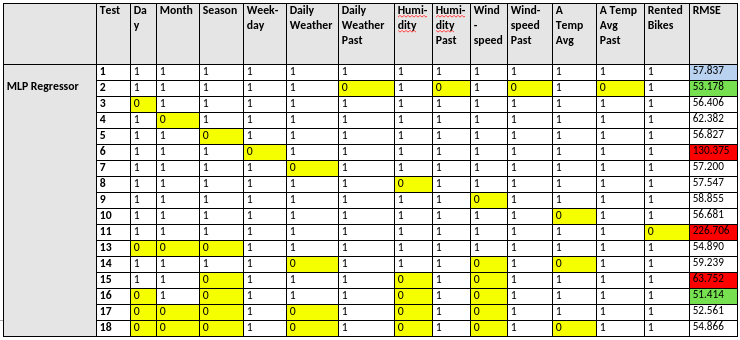
\includegraphics[width=1.2\textwidth]{img/evalmlp}\label{fig:evalmlp}
\captionof{figure}{Feature Evaluation Testcases}\label{fig:evalmlp}
\end{figure}
\subsection{Extra Features}
